\documentclass[t,aspectratio=169]{beamer}
\usetheme{metropolis}

\title{NASA Space Apps Challenge 2025:\\Build a Space Biology Knowledge Engine\\bioscholar.study}
\date{5. October 2025}
\author{Jonathan Dransfeld, Lukas Probst, Christopher von Klitzing\\Kool Intergalactic Team}
\institute{Karlsruhe Institute of Technology}

\begin{document}
\maketitle

\begin{frame}{Advanced Search}
	\begin{columns}[T]
		\begin{column}{.38\textwidth}
            \begin{itemize}
                \item Search for topics in biology
                \item Get publications and experiments matching your query
                \item Results are ranked by relevance using OpenAI text-embedding-3-small
            \end{itemize}
        \end{column}
		\begin{column}{.58\textwidth}
            
\includegraphics[width=\textwidth]{images/1_search.png}
        \end{column}
    \end{columns}
\end{frame}

\begin{frame}{Intelligent Q\&A}
	\begin{columns}[T]
		\begin{column}{.48\textwidth}
            \begin{itemize}
                \item Ask questions about the paper
                \item Get answers by OpenAI's gpt-4o-mini with context (RAG)
            \end{itemize}
            \vskip5pt
            
\includegraphics[width=\textwidth]{images/2_2_reliability.png}
        \end{column}
		\begin{column}{.48\textwidth}
            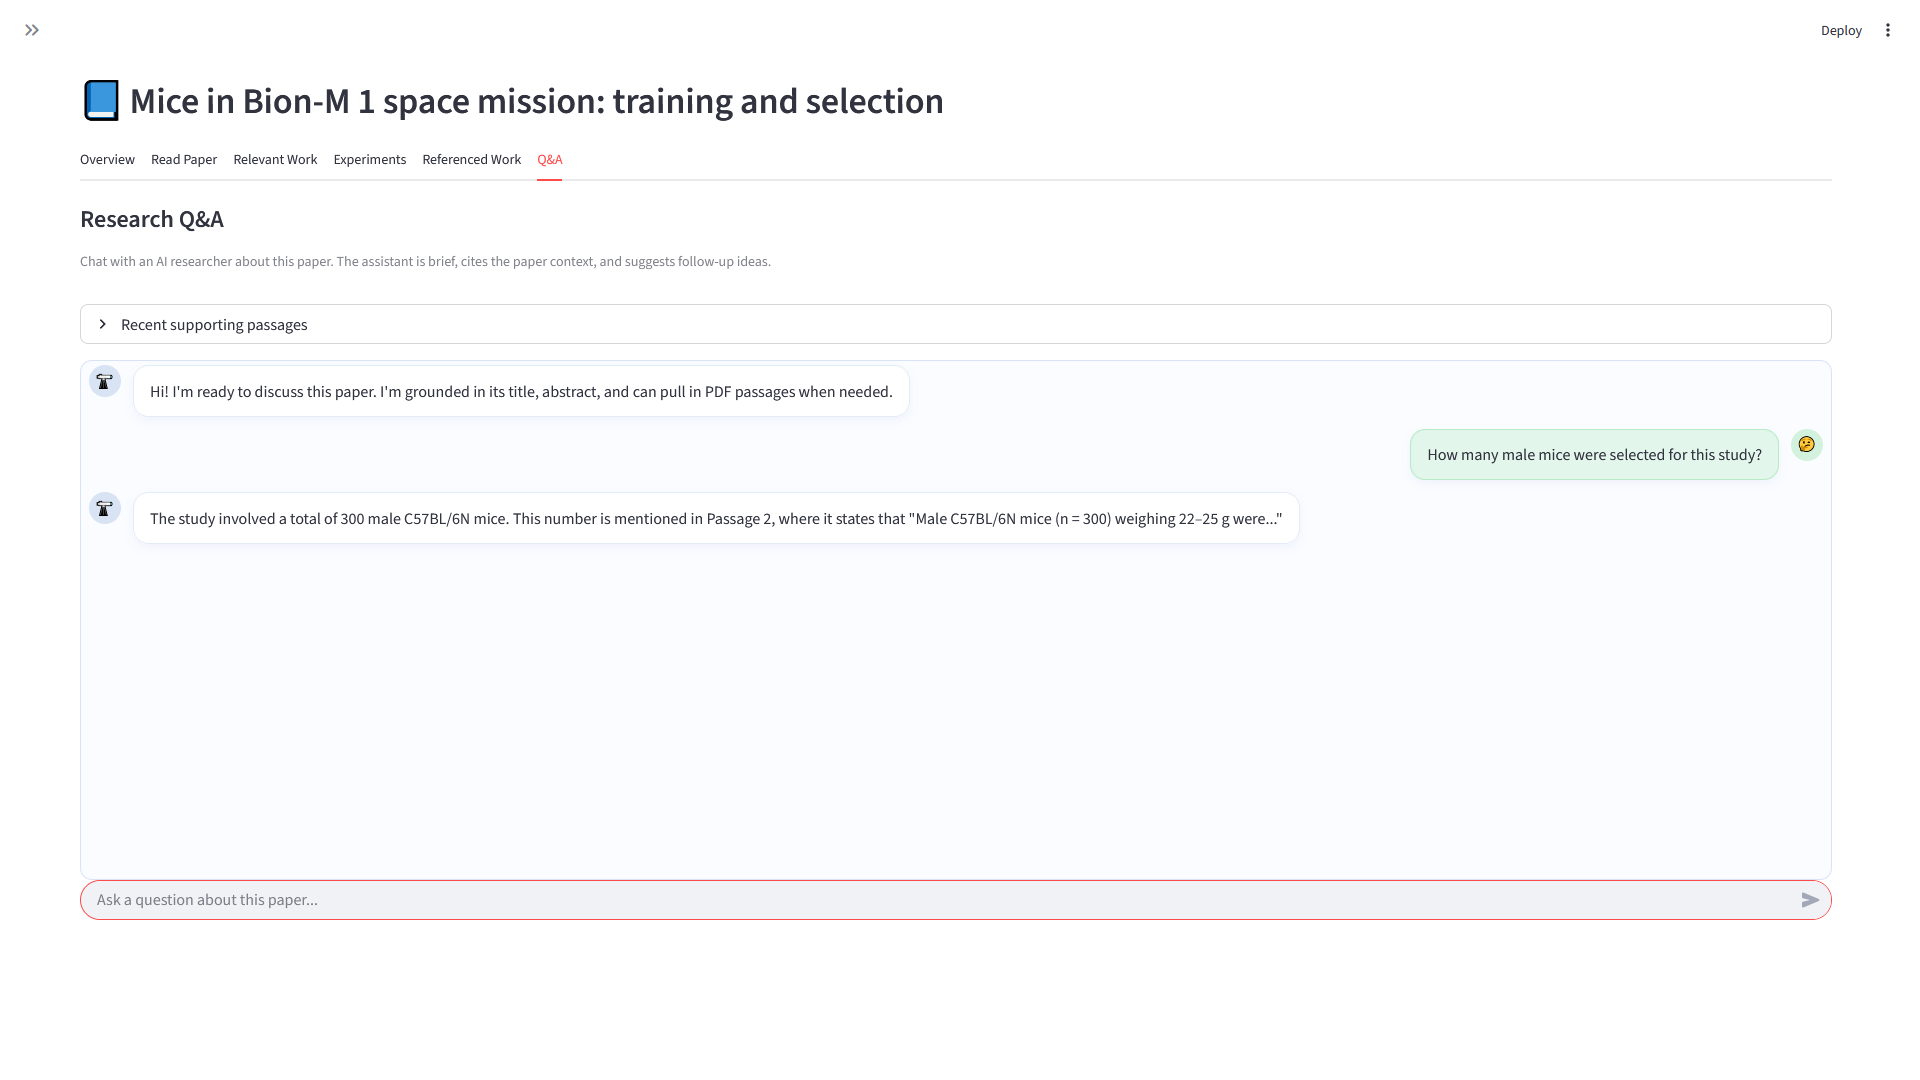
\includegraphics[width=\textwidth]{images/2_1_chat.png}
            \begin{itemize}
                \item Get supporting passages from the publication for more reliability
            \end{itemize}
        \end{column}
    \end{columns}
\end{frame}

\begin{frame}{Semantic Graph View}
	\begin{columns}[T]
		\begin{column}{.38\textwidth}
            \begin{itemize}
                \item Use of natural language processing allows for linking similar resources
                \item Allows to link arbitrary semantically related resources (like papers and experiments), making it more powerful than e.g. citations
                \item Get relevant similar resources with the use of an adapted version of Google's page rank algorithm
            \end{itemize} %
        \end{column}
		\begin{column}{.58\textwidth}
            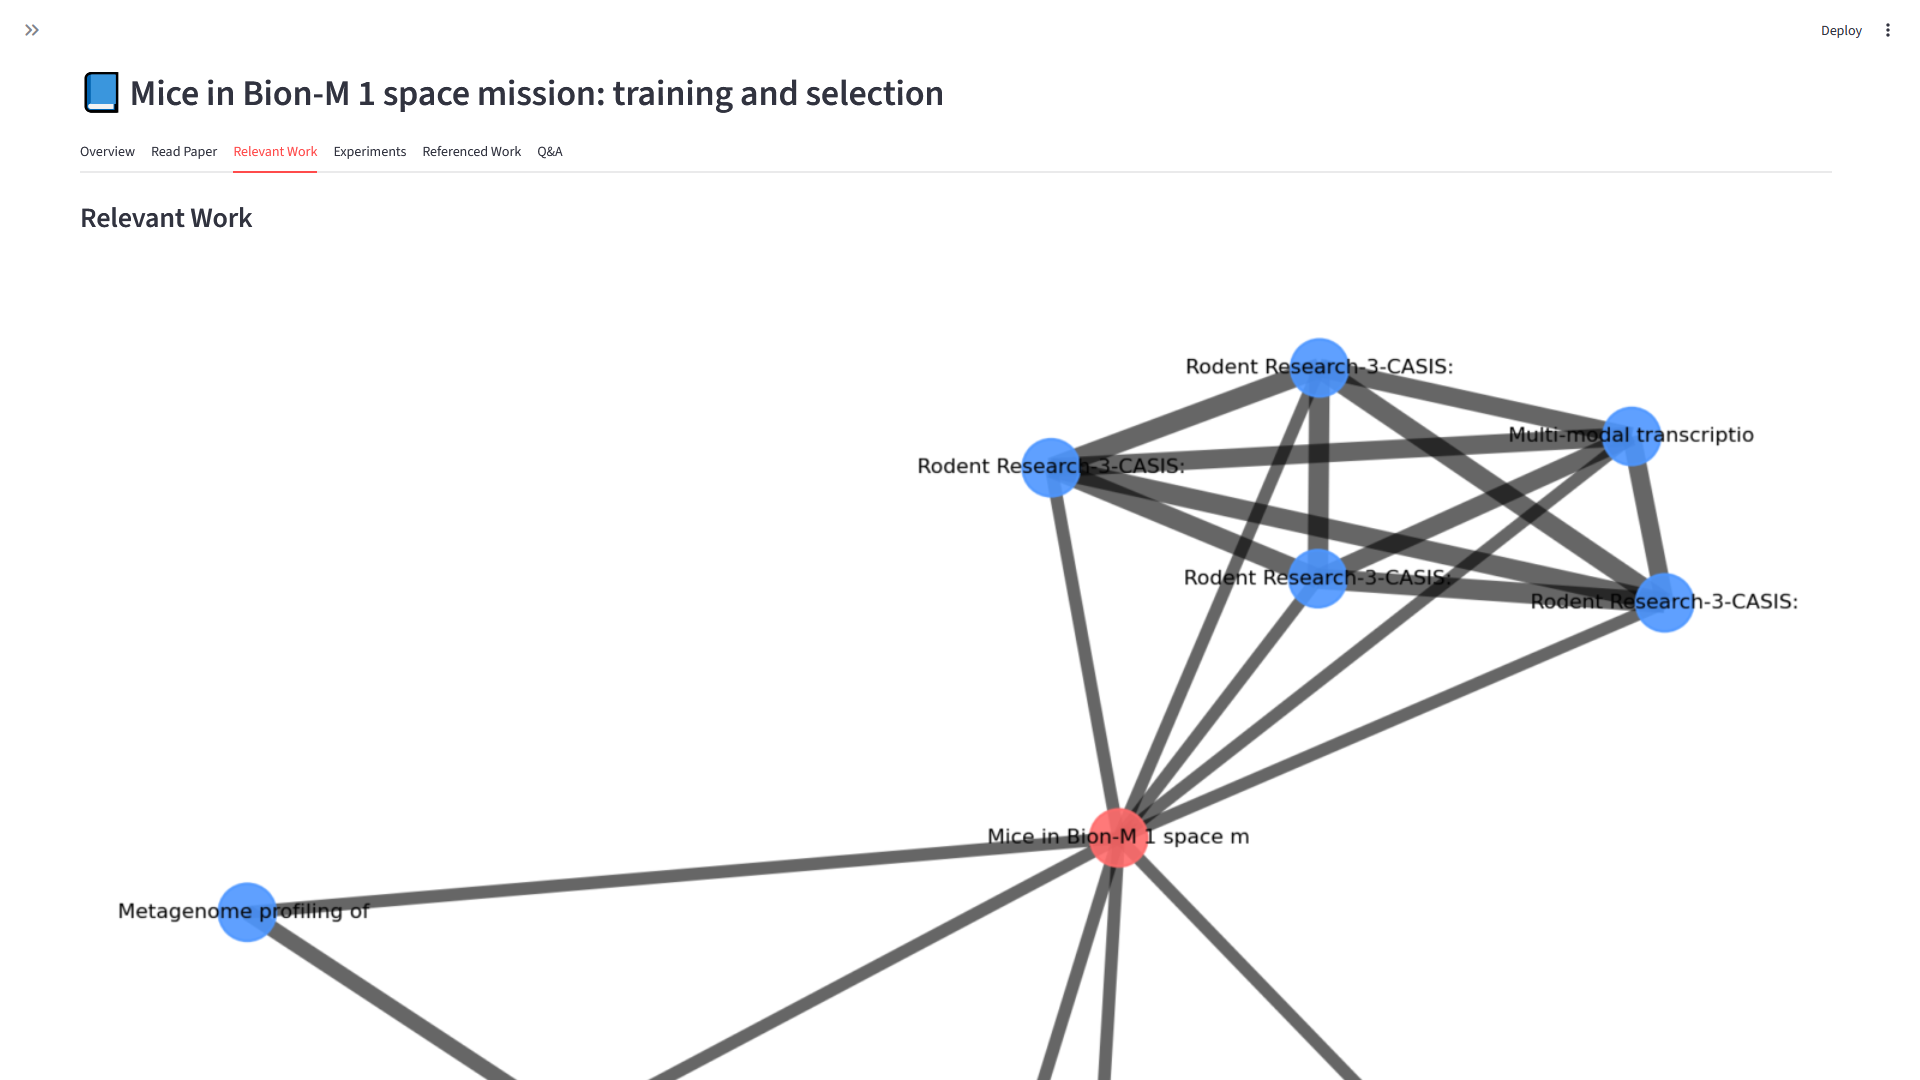
\includegraphics[width=\textwidth]{images/3_relevant_work.png}
        \end{column}
    \end{columns}
\end{frame}

\begin{frame}{Cross-Referencing}
	\begin{columns}[T]
		\begin{column}{.48\textwidth}
            \begin{itemize}
                \item BioScholar supports different types of resources, and connections between them
                \item Find publications referencing experiments\dots
            \end{itemize}
            
\includegraphics[width=\textwidth]{images/4_2_exp_to_pub.png}
        \end{column}
		\begin{column}{.48\textwidth}
            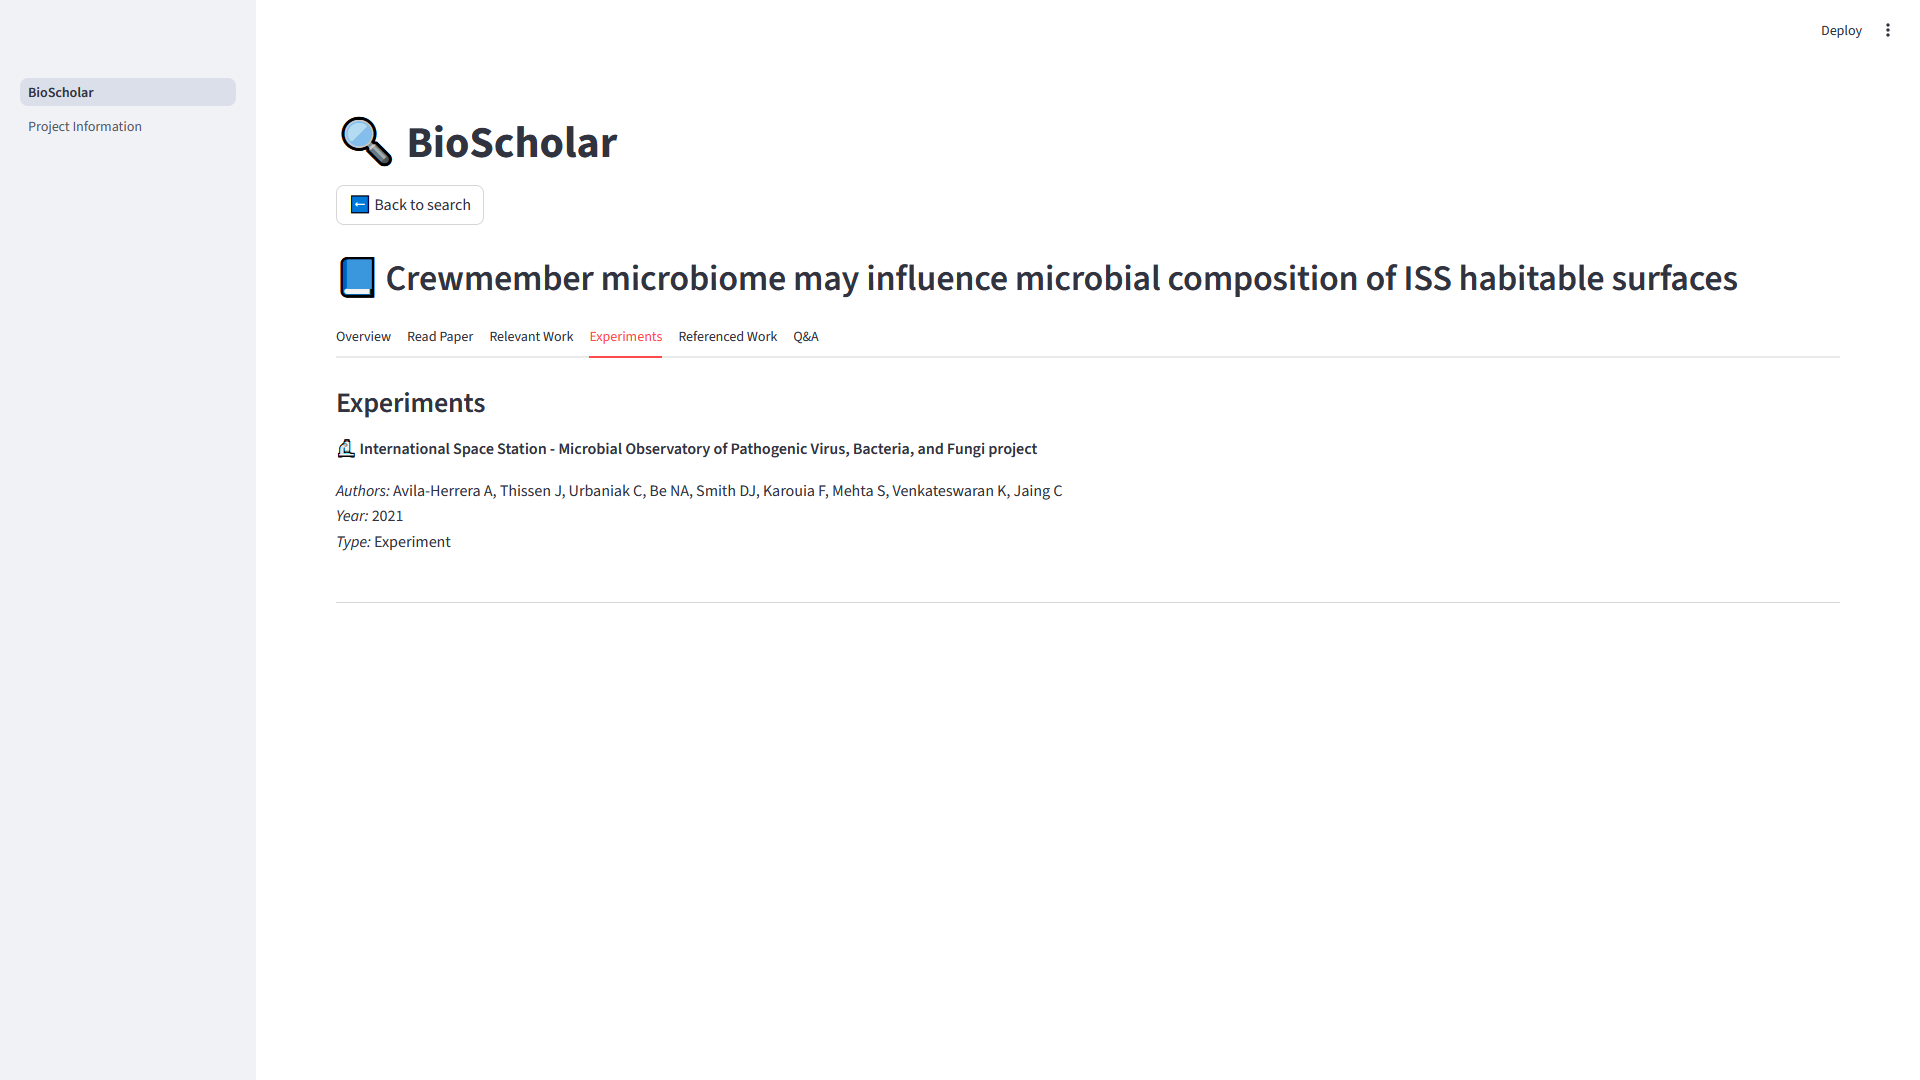
\includegraphics[width=\textwidth]{images/4_1_pub_to_exp.png}
            \begin{itemize}
                \item \dots and experiments referencing publications
            \end{itemize}
        \end{column}
    \end{columns}
\end{frame}

\begin{frame}{Integrated PDF Viewer}
	\begin{columns}[T]
		\begin{column}{.38\textwidth}
            \begin{itemize}
                \item View publications directly on BioScholar
                \item Available for all publications with a known link to a .pdf
            \end{itemize}
        \end{column}
		\begin{column}{.58\textwidth}
            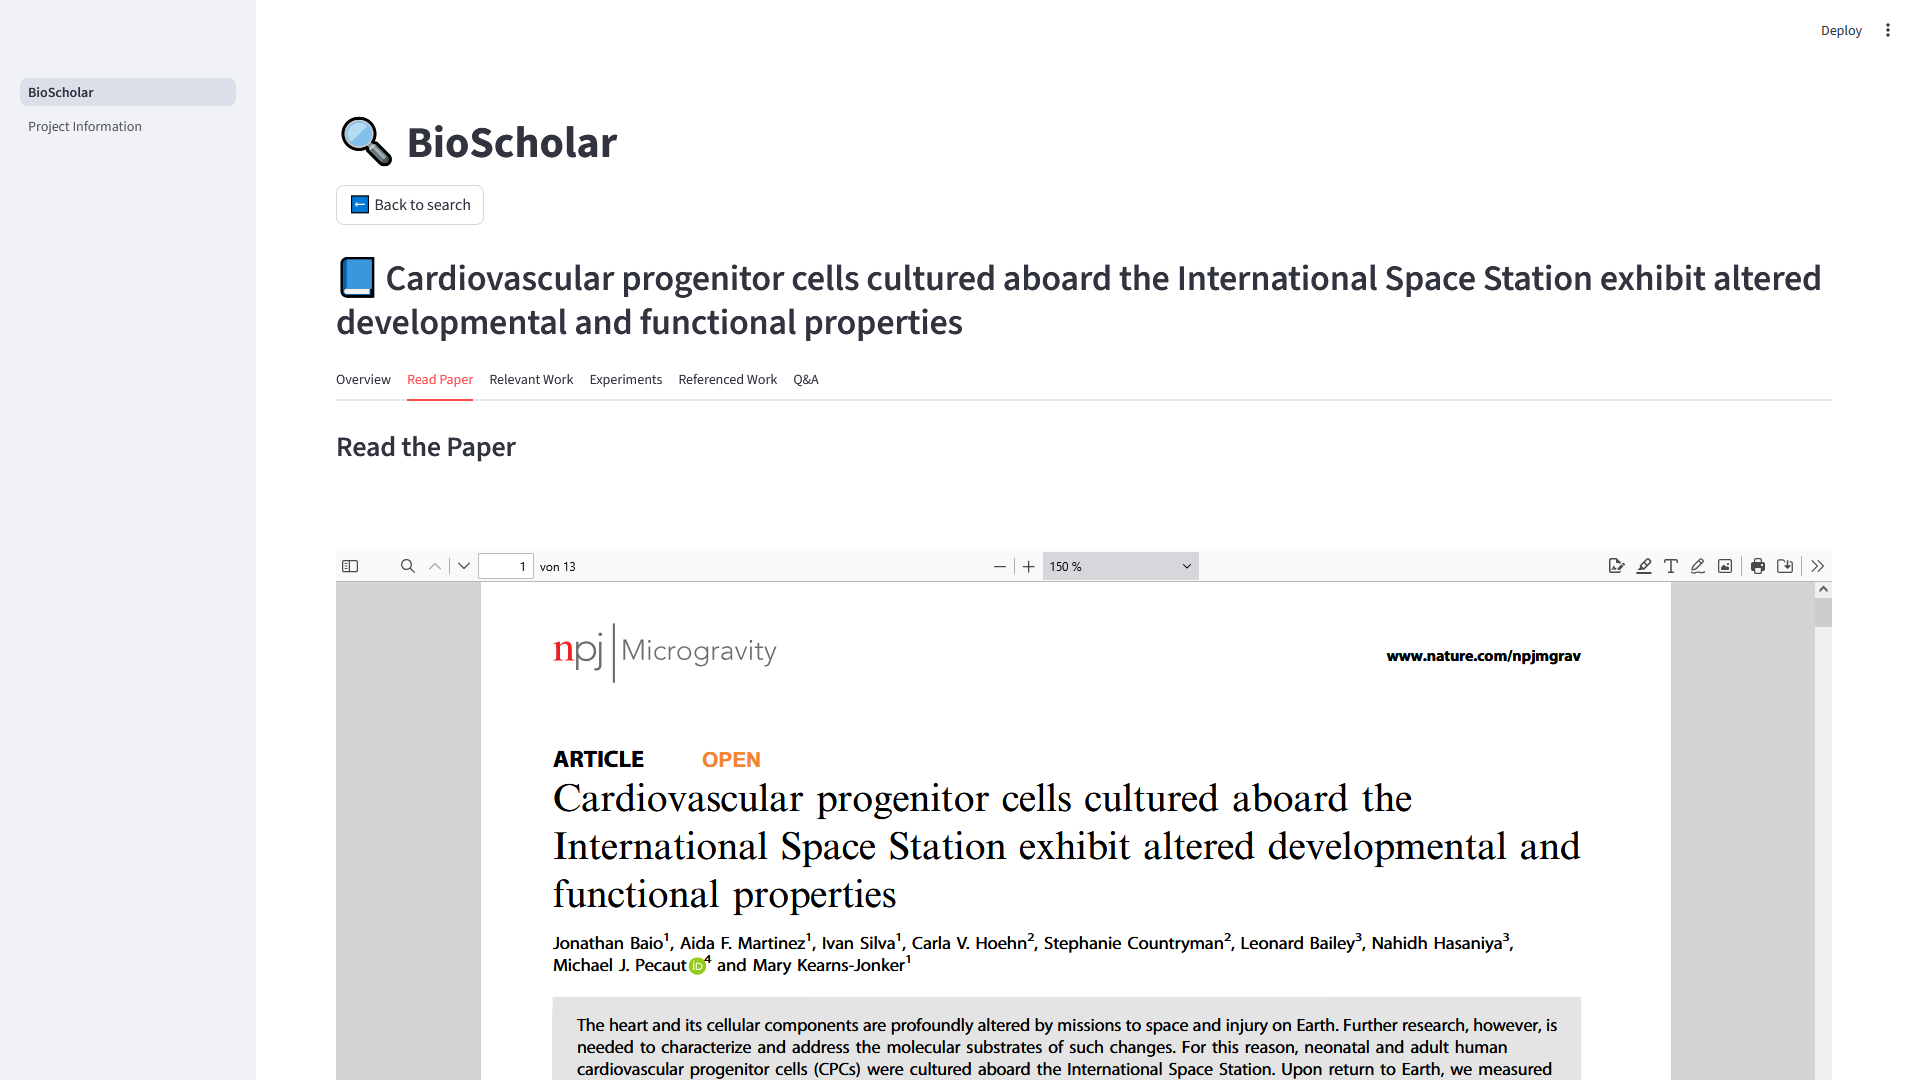
\includegraphics[width=\textwidth]{images/5_integrated_viewer.png}
        \end{column}
    \end{columns}
\end{frame}

\end{document}
